\section{LLM辅助处理与建议核验}
\label{sec:llm}

\subsection{一条建议怎样进入实际计算}
参数范围明确后，仍需要判断哪些设置值得尝试。LLM可以根据轨迹诊断提出候选，但建议本身不能说明效果：同样一句“多保留短片段”，可能改善覆盖，也可能保留较大的位置偏差。因此，建议必须转成明确参数，交给同一套工具处理，再用与确定性方案相同的参考检查。

实验使用GPT辅助讨论方法和解释结果，Codex完成实现、运行与资料整理。任务内将规划、执行和核验分成A、B、C三个职责。A依据已有证据提出比较任务；B实际计算与整理；C从原始数据和固定条件核对产物。分段、去噪和DP仍是确定性工具，不各自改名为一个模型。

\begin{figure}[H]\centering
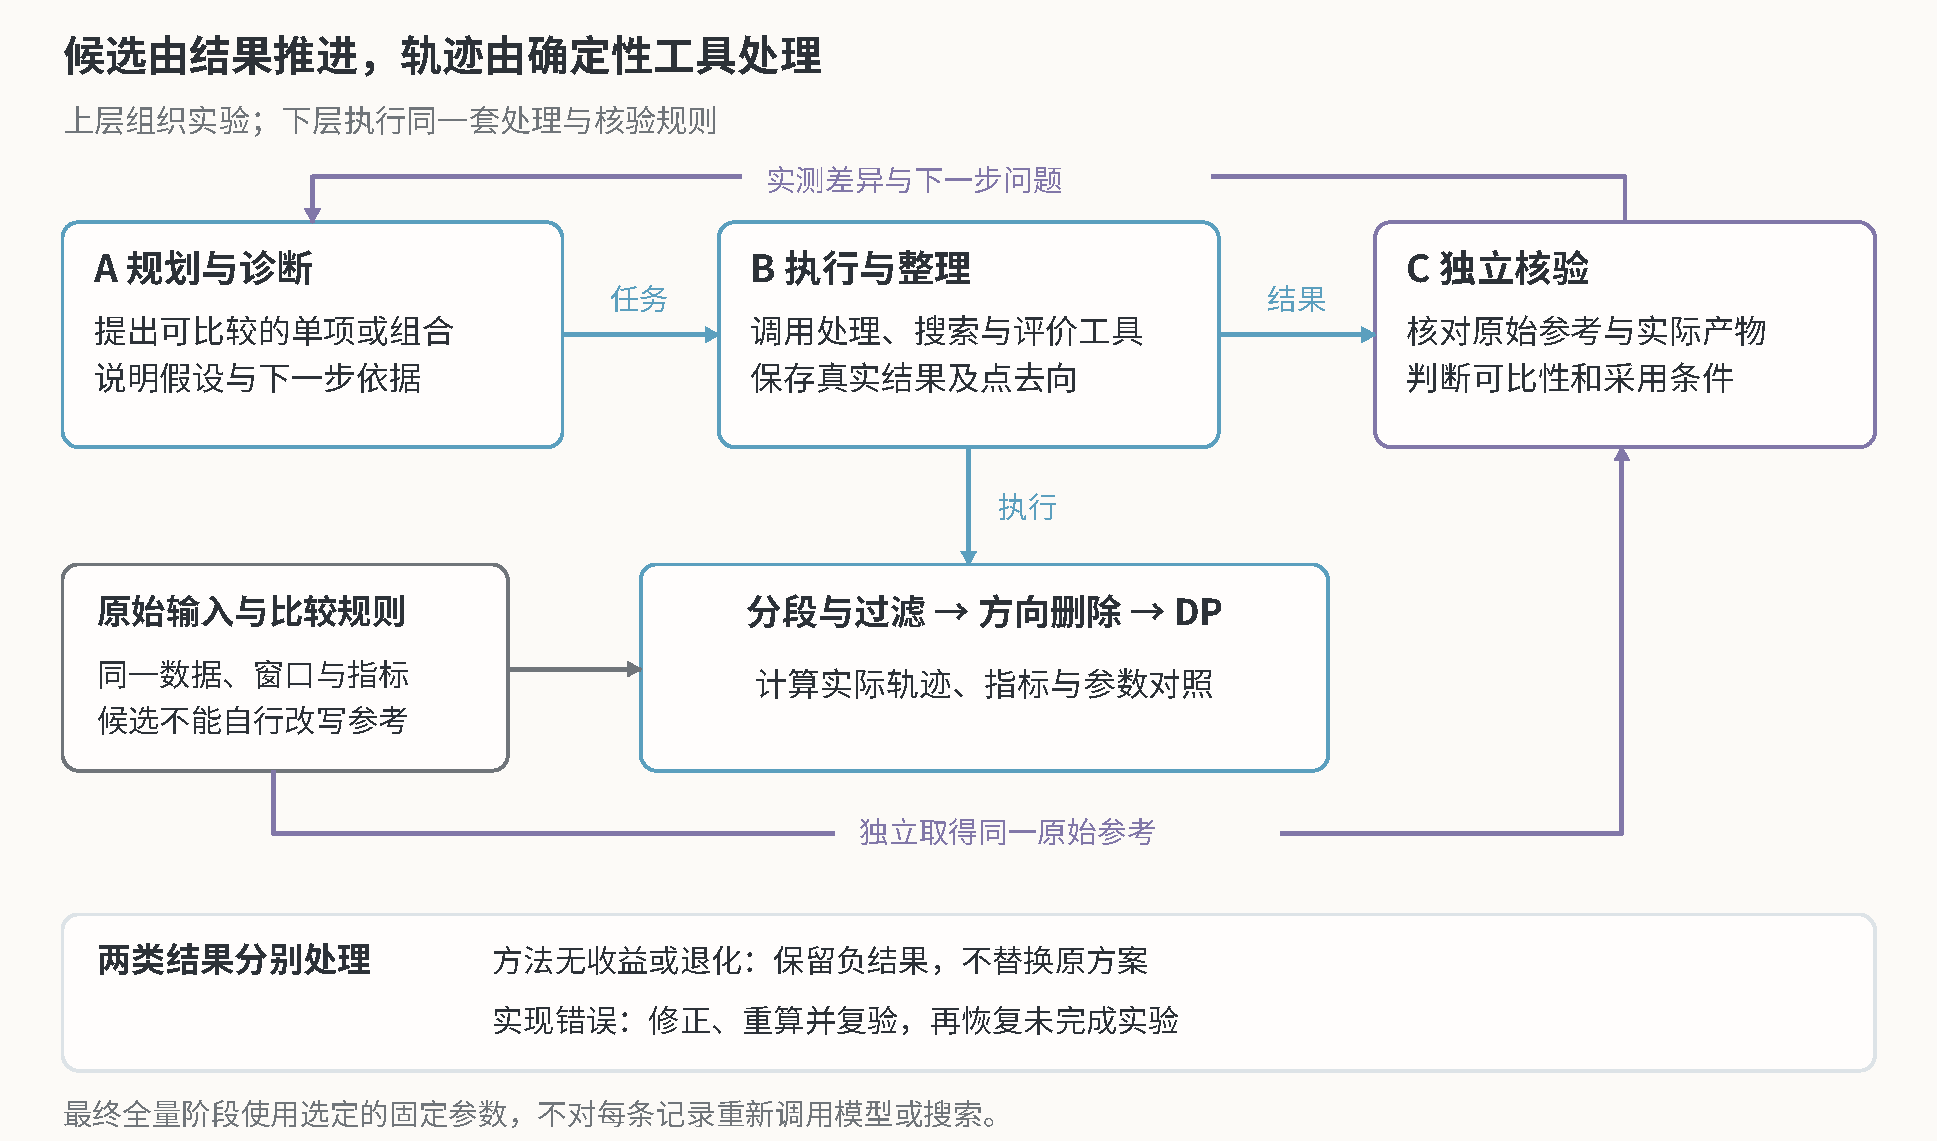
\includegraphics[width=\linewidth]{figures/workflow_structure.pdf}
\caption{实验组织与处理工具的分工。结果核验使用独立取得的原始参考，实测差异返回后续规划。方法无收益与实现错误分别处理；该结构说明实验怎样推进，不表示最终逐记录处理都调用模型。}\label{fig:workflow}
\end{figure}

角色之间传递明确的输入范围、参数、输出和检查结论，而不是只有“帮我优化”的自然语言。执行出错时先修正实现，重新计算受影响结果，再恢复原比较；候选正确执行但无收益时保留负结果，不把它当作必须修到胜出的故障。普通动作在已有范围内完成，改变方法含义或比较目标的问题才需要重新讨论。

这一组织方式服务于整个实验的推进。下面的四模式则比较\textbf{记录级参数决策}怎样使用模型、反馈和记忆，两者不混为一项：治理角色参与代码或报告，不计入“仅确定性搜索”的记录级调用。

\subsection{四种运行方式分别能看到什么}
一次建议是否足够，实测反馈是否有帮助，需要通过不同权限的模式比较。表\ref{tab:mode-definition}列出各模式的差别。它们使用相同数据、基础工具与参数范围，但不强行拥有相同的信息。

\begin{table}[htbp]\centering\small
\caption{四种模式的决策条件}\label{tab:mode-definition}
\begin{tabularx}{\linewidth}{@{}L{32mm}YY@{}}\toprule
模式 & 决策可见信息 & 实际动作\\\midrule
仅LLM建议 & 原始诊断卡、方法和合法参数域 & 一次提议锁定后执行；评分不回传修改该提议\\
仅确定性搜索 & 共同设置及本模式的工具结果 & 按预登记20项配置序列搜索；零记录级模型调用\\
LLM＋搜索 & 原始诊断和自己的实测反馈 & 最多3轮；提出候选、执行、再据结果调整或停止\\
LLM＋记忆＋搜索 & 同上，加冻结示范记忆 & 相同回合与候选上限，额外读取适用经验\\\bottomrule
\end{tabularx}
\end{table}

搜索型模式每条记录最多评价20个候选，反馈轮次的累计上限依次为8、14、20；允许提前停止，所以上限相同不意味着实际计算量相同。仅LLM模式没有搜索机会，不称为等计算量实验。确定性搜索遍历固定序列，LLM可在设定的六参数离散域内提出完整向量；比较的是这些明确策略，而不是完全隔离所有搜索差异后的模型能力。

诊断卡只含必要原始统计，不把完整坐标序列直接塞入模型。每次真实派发最多包含8张卡，分别保存建议与结果。原样建议先接受合法性检查，不先夹到合法范围再统计成功。允许反馈的模式可在剩余预算内修改；仅LLM不能获得隐藏的二次修正。

开发比较采用同一24条记录、各1次独立运行；阶段评估采用另一组共同24条记录、各3次独立运行。表\ref{tab:modes}中的72为$24\times3$次记录观察，不是72条互不相关的轨迹。各次会话与工作记忆重置，模型统一使用\texttt{gpt-6-astra}（medium设置），未固定随机种子。

\begin{table}[htbp]\centering\small
\caption{真实四模式的结果与实际计算量}\label{tab:modes}
\begin{tabular}{@{}llrrrr@{}}\toprule
分区 & 模式 & 改善 / 观察 & 候选评价 & 模型派发 & 批次总时长/秒\\\midrule
开发 & 仅LLM建议 & 8/24 & 36 & 3 & 113.2\\
开发 & 仅确定性搜索 & 9/24 & 480 & 0 & 30.8\\
开发 & LLM＋搜索 & 16/24 & 372 & 9 & 320.8\\
开发 & LLM＋记忆＋搜索 & 17/24 & 330 & 9 & 297.0\\\midrule
阶段评估 & 仅LLM建议 & 15/72 & 109 & 9 & 324.4\\
阶段评估 & 仅确定性搜索 & 27/72 & 1,440 & 0 & 88.6\\
阶段评估 & LLM＋搜索 & 47/72 & 1,080 & 27 & 1,007.0\\
阶段评估 & LLM＋记忆＋搜索 & 47/72 & 954 & 27 & 892.1\\\bottomrule
\end{tabular}
\tabnote{改善指锁定输出通过全部规定保护并有严格改善，不是真实噪声识别成功率。候选评价包含工具参照等实际计量范围；仅LLM的独立参照评价不进入其决策反馈。时间是批次墙钟时间之和，不是每条轨迹的延迟。}
\end{table}

两种允许模型读取反馈的模式，在这组阶段评估中得到较多符合比较条件的输出，但也消耗了更多模型回合。相同记录的重复不是额外独立样本，这些计数不能单独证明任意数据上的总体优势。有效实验共84次可见模型派发；没有用模型调用次数本身作为质量指标。

\subsection{示范记忆是否影响建议与结果}
若经验条目来自待评估记录本身，模型可能只是找回已经知道的答案。因此，情景记忆只用60条独立示范记录建立，并经工具核验后保存。26条在规定比较中获得支持，34条没有新增收益；无收益经验也保留其性质，不改名为成功案例。

检索依据六个原始特征：点数、空间跨度、正时间差中位数的$\log(1+x)$，以及零时间差、重复位置、原始断点比例。尺度只由示范集固定；在相同描述层内取最多3个近邻，排除本记录和已知关联来源。当前运行的短期记录与示范长期记忆分开，评估阶段不写回，也没有另行填入未经来源说明的人类知识条目。

\begin{table}[htbp]\centering\small
\caption{记忆作用的不同观察层次}\label{tab:memory}
\begin{tabularx}{\linewidth}{@{}L{42mm}L{27mm}Y@{}}\toprule
观察对象 & 实际读数 & 能说明什么\\\midrule
带记忆的记录观察收到条目 & 96/96 & 信息实际送入相应上下文\\
决策回合引用有效条目 & 60/241 & 存在可追踪的引用\\
回合满足动作一致判定 & 49/241 & 部分参数与引用内容一致\\\bottomrule
\end{tabularx}
\end{table}

送达、引用和建议变化是不同层次，不能互换分母，也不自动构成质量收益。阶段评估中，带记忆和不带记忆的搜索模式均有47/72个符合条件的输出，但候选和各次运行仍有差异。当前结果既不足以证明记忆的因果质量增益，也不足以证明所有情形等效。最终采用统一参数，不要求在全量处理时逐条重复检索。

\subsection{局部检查合格，为什么仍未采用}
一个具体建议更能说明核验怎样决定取舍。对记录7764，带记忆搜索提出进一步增加空间切分、放宽短段过滤的设置：时间30秒、距离200工作米、最少2点、最短长度0、方向60度、DP容差5工作米。建议同时指出覆盖与保真仍需实测。

参数可以执行，原有122点覆盖也保持不变。但在同一覆盖集合上，最大几何偏差从40.215增至69.145工作米；候选的P即时误差约4.826工作米，仍小于5。它说明\textbf{简化步骤合格，不等于完整处理结果优于参考}，因此该候选没有作为当前采用结果。图\ref{fig:g6}把输入、两条处理路径和不同检查之间的关系展开。

后续使用方向60度、DP容差2的另一提议虽然降低了自身P误差，共同最大偏差仍为42.546工作米，未优于参考。另一个进一步切分的提议丢失了11个原有覆盖点，先违反覆盖条件，此时也不能直接拿不同覆盖集合的最大误差作配对增减。

真实建议并非都无效。记录10232的建议预期方向删除减少，实测由32点降到10点，差值为$-22$，共同最大偏差也降低。预测方向正确、某记录满足比较条件，与跨记录的统一方法成立仍是不同结论。

\FloatBarrier
\begin{landscape}
\thispagestyle{empty}
\noindent{\sffamily\small\color{Muted}智慧城市与位置服务\hfill Experiment Report}\par
\vspace{3mm}
\begin{figure}[H]\centering
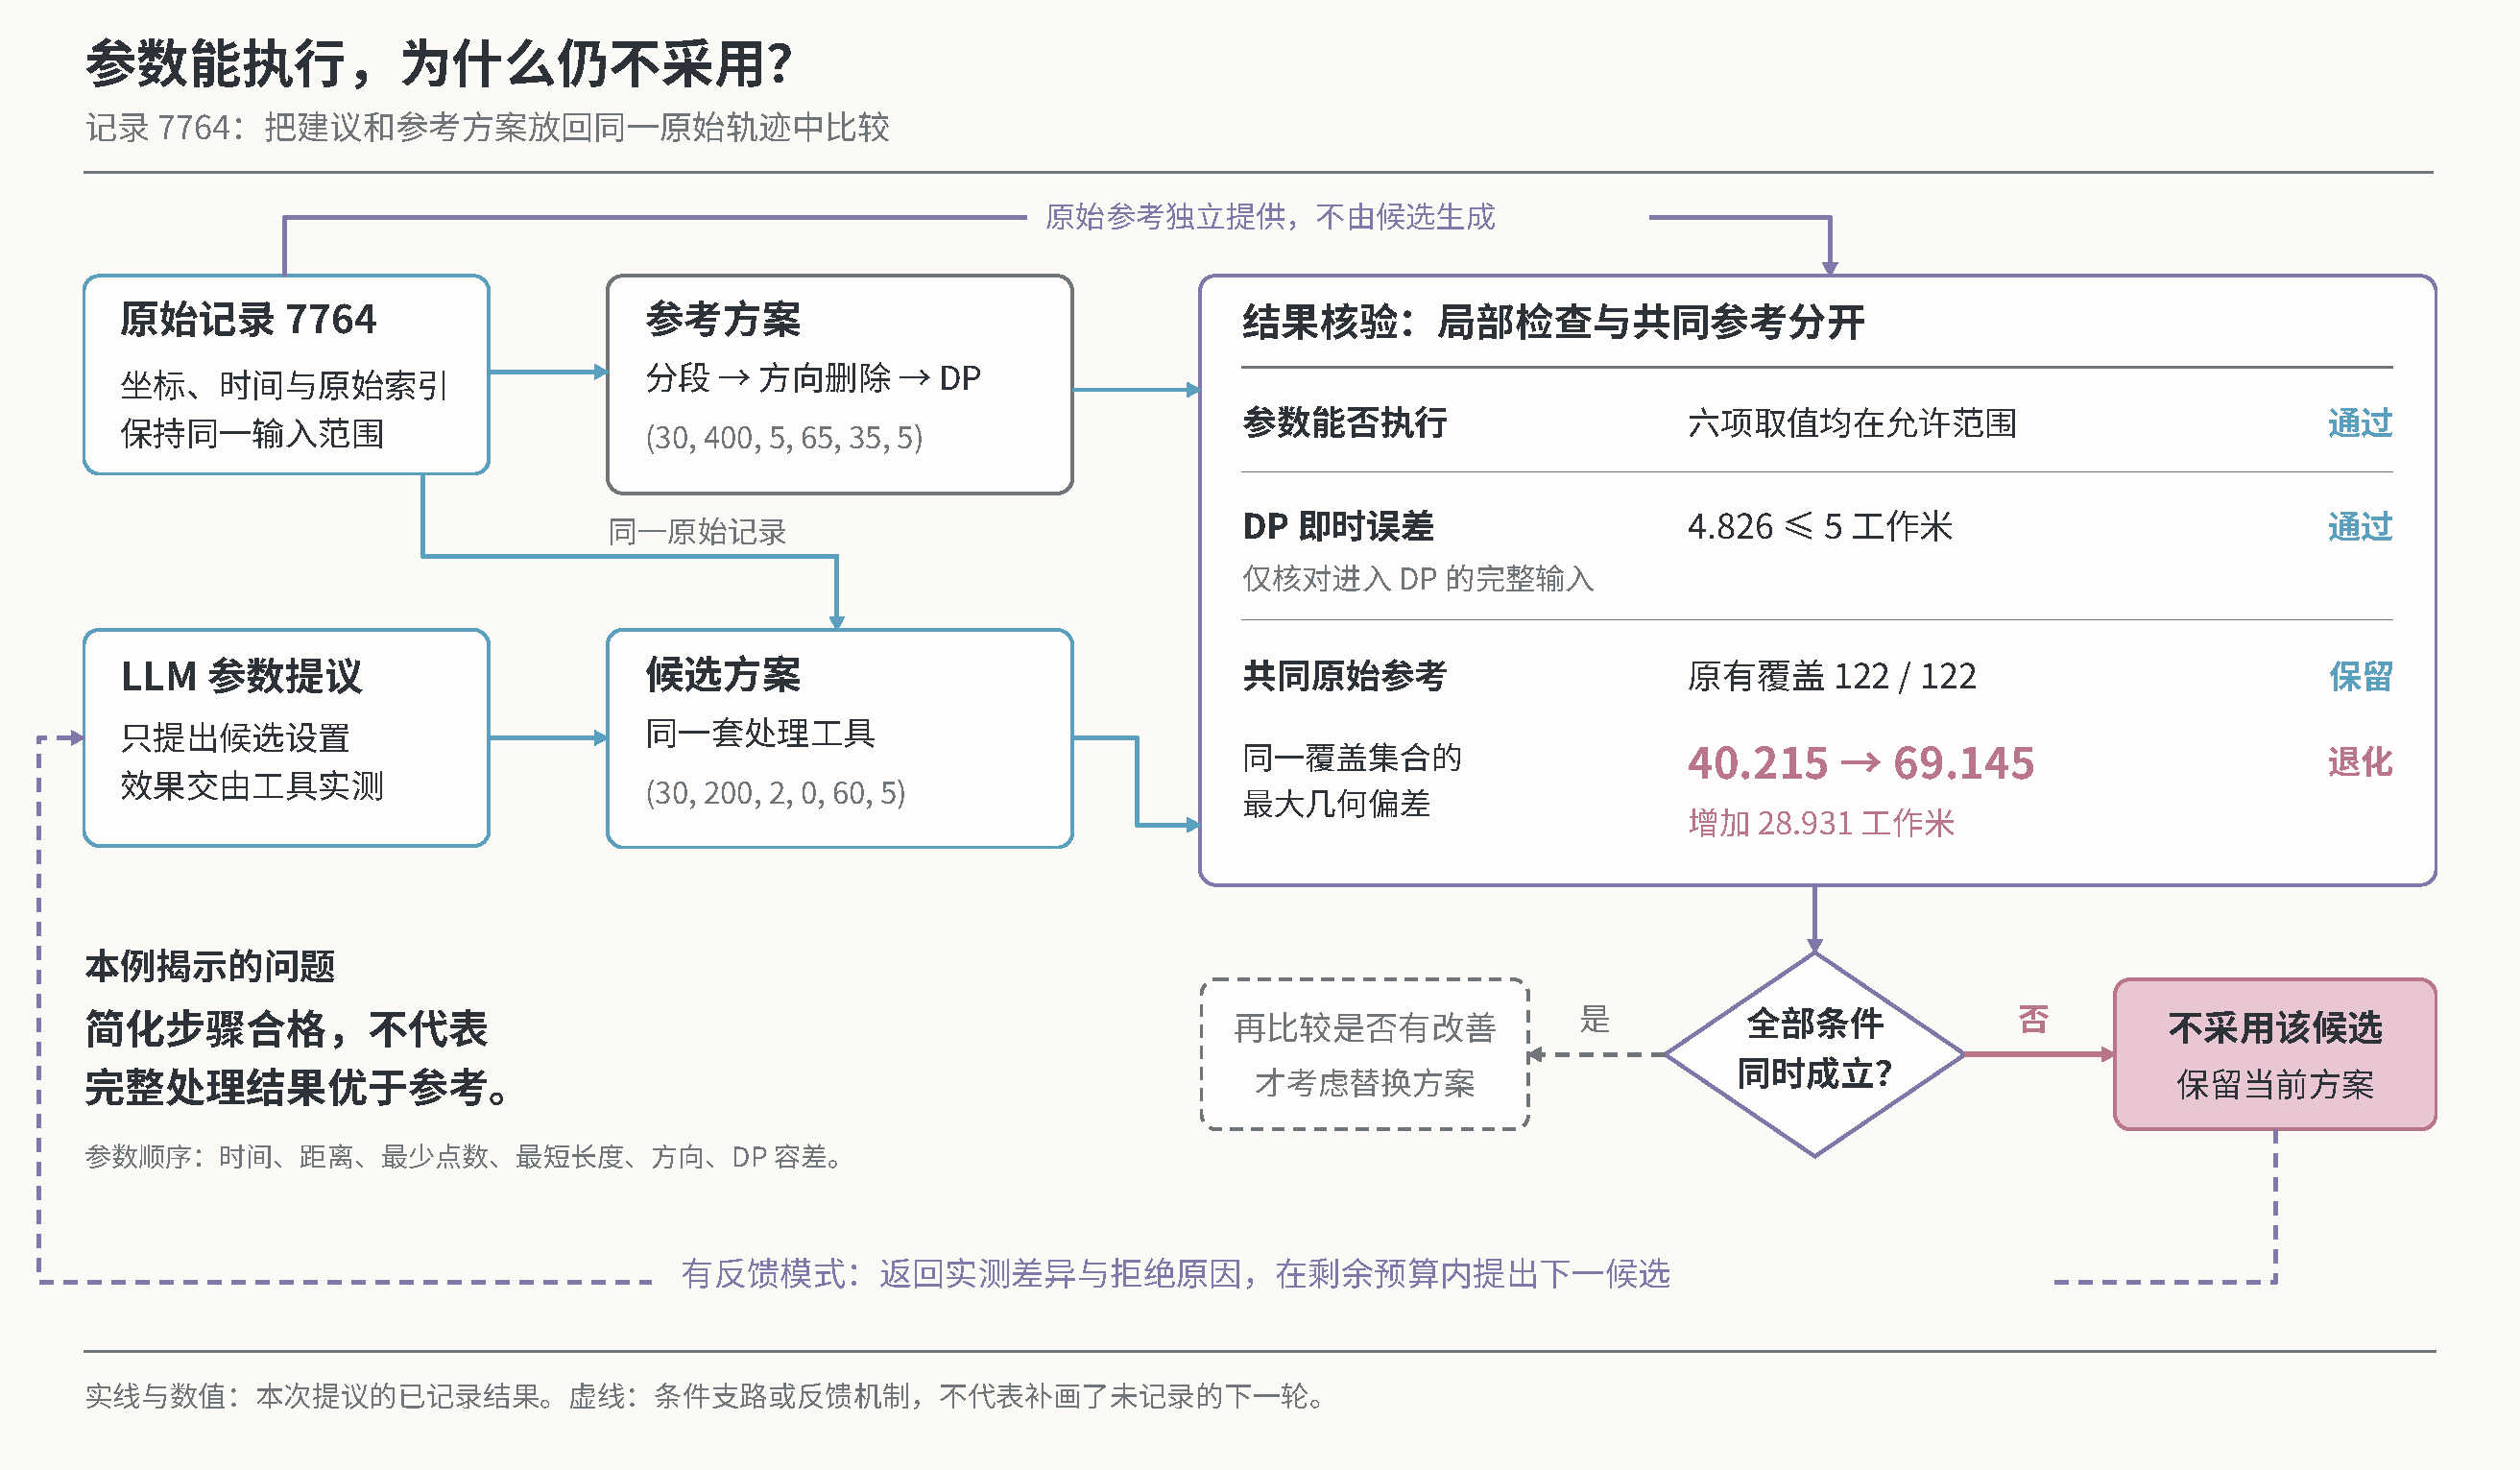
\includegraphics[width=.92\linewidth]{figures/G6A_verification_logic.pdf}
\caption{记录7764的建议核验。原始输入分别供给参考处理、候选处理及独立评价；参数、P即时误差和共同原始几何分开检查。虚线只表示有反馈模式可采用的后续机制，不表示本例发生了图中未列出的新一轮调用。}\label{fig:g6}
\end{figure}
\end{landscape}

\subsection{反例揭示了哪些隐含假设}
真实数据没有噪声真值，不能据删除数量计算误删率。为检查具体数学机制，实验另构造具有已知答案的小型轨迹。表\ref{tab:counterexamples}列出实际运行结果；这些答案仅适用于各自构造，不转移成真实数据标签。

\begin{table}[htbp]\centering\small
\caption{已知答案反例的实测结果与对应认识}\label{tab:counterexamples}
\begin{tabularx}{\linewidth}{@{}L{24mm}Y Y@{}}\toprule
检查问题 & 实际处理结果 & 说明什么\\\midrule
方向与噪声 & 5点正常折返删除2点；5点尖峰删除2点，其中1个预设噪声、1个正常点 & 方向突变不能唯一识别噪声；直角例5点全留也不证明所有转弯安全\\
零值与缺失 & 5点4边中，2条零时间差速度不可用，1条零位移方向不可用 & 不能用速度0、方向0替代不可计算；窗口按定义保留\\
先P后S & 时间间隔例中S-D-P保留4/5点、覆盖100\%；P-S-D无输出 & P即时省点率60\%不能掩盖最终覆盖为0\\
隐藏空间断点 & 两种顺序均留2/3点，P-S-D却有1条跨原始断点边 & 相同点数和覆盖率不足以证明连接关系相同\\
有限线段与等号 & 越界投影距离为$\sqrt2$，正确DP留3点；误差与容差均为1时留2点 & 用有限线段而非延长直线；严格超过才递归\\
全部过滤 & 原始3点仍计入分母，覆盖为0，误差与P省点率不可用 & 无输出不能成为“零误差”的赢家\\
不同clean自证 & 两种方向设置的自身P误差都为0，共同原始最大偏差为0.447214和0 & 各自输入上的低误差不能代替共同参考\\\bottomrule
\end{tabularx}
\end{table}

同理，缺失期间线性插值隐含连续、近似匀速直线运动，但采样空档可能包含停留、转弯或未知路径。实验没有用无依据插值补造轨迹。课程要求的AI批判\cite{teacher}在这里落实为可检查的假设、实际反例与取舍，而不是仅说“不要相信模型”。

基础方法和LLM提议经过相同的处理与评价，保留正例，也保留合法但退化的结果。接下来关注另一个问题：已有单项调整结合后，是否真的带来额外作用。
